\documentclass[12pt,a4paper]{report}

% ── Packages ──────────────────────────────────────────────────────────────────
\usepackage[a4paper, margin=2.5cm, top=3cm, bottom=3cm]{geometry}
\usepackage[T1]{fontenc}
\usepackage[utf8]{inputenc}
\usepackage{xcolor}
\usepackage{graphicx}
\usepackage{booktabs}
\usepackage{array}
\usepackage{tabularx}
\usepackage{colortbl}
\usepackage{enumitem}
\usepackage{parskip}
\usepackage{titlesec}
\usepackage{fancyhdr}
\usepackage{hyperref}
\usepackage{tcolorbox}
\usepackage{amsmath}
\usepackage{caption}
\usepackage[nottoc]{tocbibind}

% ── Colours ───────────────────────────────────────────────────────────────────
\definecolor{darkblue}{HTML}{1F4E79}
\definecolor{medblue}{HTML}{2E74B5}
\definecolor{lightblue}{HTML}{D6E4F0}
\definecolor{altrow}{HTML}{EBF3FB}
\definecolor{greenbg}{HTML}{E2EFDA}
\definecolor{headerbg}{HTML}{1F4E79}
\definecolor{statusgreen}{HTML}{70AD47}
\definecolor{statusamber}{HTML}{FFC000}

% ── tcolorbox ─────────────────────────────────────────────────────────────────
\tcbuselibrary{skins, breakable}

\newtcolorbox{deliverablebox}[1]{
  colback=greenbg, colframe=darkblue, coltitle=white,
  fonttitle=\bfseries, title={#1},
  breakable, boxrule=0.8pt, arc=3pt,
  left=6pt, right=6pt, top=4pt, bottom=4pt
}
\newtcolorbox{infobox}{
  colback=lightblue!60, colframe=medblue,
  boxrule=0.6pt, arc=2pt,
  left=6pt, right=6pt, top=3pt, bottom=3pt
}

% ── Caption style ─────────────────────────────────────────────────────────────
\captionsetup{font=small, labelfont=bf, labelsep=period}

% ── Section formatting ────────────────────────────────────────────────────────
\titleformat{\chapter}[block]
  {\Large\bfseries\color{darkblue}}{\thechapter.}{0.6em}{}
  [\color{medblue}\titlerule]
\titleformat{\section}[block]
  {\large\bfseries\color{medblue}}{\thesection}{0.5em}{}
\titleformat{\subsection}[block]
  {\normalsize\bfseries\color{darkblue!80}}{\thesubsection}{0.5em}{}
\titlespacing*{\chapter}{0pt}{12pt}{10pt}
\titlespacing*{\section}{0pt}{10pt}{6pt}
\titlespacing*{\subsection}{0pt}{8pt}{4pt}

% ── Header / Footer ───────────────────────────────────────────────────────────
\pagestyle{fancy}
\fancyhf{}
\renewcommand{\headrulewidth}{0.4pt}
\renewcommand{\footrulewidth}{0.4pt}
\fancyhead[L]{\small\color{darkblue}\textbf{Phase 1 Completion Report}}
\fancyhead[R]{\small\color{darkblue}Rajib Roy --- 24459 $|$ IISc M.Tech (AI)}
\fancyfoot[C]{\small\thepage}
\fancyfoot[R]{\small\color{gray}April 2026}

% ── Hyperref ──────────────────────────────────────────────────────────────────
\hypersetup{colorlinks=true, linkcolor=medblue, urlcolor=medblue,
  pdftitle={Phase 1 Completion Report --- Rajib Roy}, pdfauthor={Rajib Roy}}

% ── Table column types ────────────────────────────────────────────────────────
\newcolumntype{L}[1]{>{\raggedright\arraybackslash}p{#1}}
\newcolumntype{C}[1]{>{\centering\arraybackslash}p{#1}}

% ── Status macros ─────────────────────────────────────────────────────────────
\newcommand{\statuscomplete}{\colorbox{statusgreen}{\color{white}\textbf{\small Complete}}}
\newcommand{\statusphase}[1]{\colorbox{statusamber}{\color{white}\textbf{\small #1}}}

% ── Lists ─────────────────────────────────────────────────────────────────────
\setlist[itemize]{leftmargin=1.4em, itemsep=3pt, topsep=4pt}
\setlist[enumerate]{leftmargin=1.4em, itemsep=3pt, topsep=4pt}

% ── Graphics path ─────────────────────────────────────────────────────────────
\graphicspath{{figs/}}

% ═════════════════════════════════════════════════════════════════════════════
\begin{document}
\pagenumbering{roman}

% ── COVER PAGE ────────────────────────────────────────────────────────────────
\begin{titlepage}
  \thispagestyle{empty}
  \begin{center}
    \vspace*{1cm}
    {\large\color{darkblue}M.Tech.\ (Online) --- Artificial Intelligence}\\[4pt]
    {\large\color{darkblue}Indian Institute of Science, Bangalore}\\[2cm]
    {\Huge\bfseries\color{darkblue}PHASE 1 COMPLETION REPORT}\\[1cm]
    {\color{medblue}\rule{\linewidth}{2pt}}\\[0.5cm]
    {\LARGE\bfseries\color{medblue}
      Detection of AI-Generated and Cloned Speech\\[6pt]
      to Strengthen Voice-Based Authentication\\[6pt]
      in Banking Environments}\\[0.4cm]
    {\color{medblue}\rule{\linewidth}{1pt}}\\[1.8cm]
    \begin{tabular}{@{}L{4.5cm}L{9cm}@{}}
      \rowcolor{lightblue}\textbf{Student Name}   & Rajib Roy \\
      \rowcolor{white}    \textbf{Student Number} & 24459 \\
      \rowcolor{lightblue}\textbf{Programme}      & M.Tech.\ in Artificial Intelligence \\
      \rowcolor{white}    \textbf{Internal Guide} & Dr.\ Anil Rahate, Practice Head --- AI, Wipro Ltd \\
      \rowcolor{lightblue}\textbf{IISc Mentor}    & Prof.\ Chandra Sekhar Seelamantula,
                                                     Dept.\ of Electrical Engineering, IISc \\
      \rowcolor{white}    \textbf{Phase Covered}  & Phase 1 \quad (January 2026 --- April 2026) \\
      \rowcolor{lightblue}\textbf{Report Date}    & April 2026 \\
    \end{tabular}
  \end{center}
\end{titlepage}

\tableofcontents
\listoffigures
\clearpage
\pagenumbering{arabic}

% ═════════════════════════════════════════════════════════════════════════════
\chapter{Executive Summary}
% ═════════════════════════════════════════════════════════════════════════════

This report documents the completion of \textbf{Phase 1} of the M.Tech.\ project titled
\textit{Detection of AI-Generated and Cloned Speech to Strengthen Voice-Based Authentication
in Banking Environments}. Phase 1 covered January 2026 -- April 2026 and comprised three
formal deliverables as defined in the approved project proposal: a literature review and
benchmark survey, a curated dataset, and a modular feature-extraction pipeline.

\textbf{All three Phase 1 deliverables have been completed on schedule.}

\medskip
\begin{center}
\begin{tabular}{L{4.2cm}L{6.8cm}C{2cm}}
  \toprule
  \rowcolor{headerbg}
  \color{white}\textbf{Deliverable} &
  \color{white}\textbf{Outcome} &
  \color{white}\textbf{Status} \\
  \midrule
  Literature review \& benchmark survey &
  Comprehensive survey: ASVspoof series, classical and deep learning anti-spoofing methods,
  robustness and domain-mismatch findings &
  \statuscomplete \\[4pt]
  \rowcolor{altrow}
  Dataset construction \& preprocessing &
  17{,}947 utterances from 10 sources; 8\,kHz + G.711 simulation; speaker- and
  system-independent splits; Edge-TTS hold-out established &
  \statuscomplete \\[4pt]
  Feature extraction pipeline &
  257-dimensional handcrafted feature vectors and 128-bin log-Mel spectrograms;
  modular Python scripts with \texttt{config.yaml} reproducibility &
  \statuscomplete \\
  \bottomrule
\end{tabular}
\end{center}

\medskip
The completed Phase 1 artefacts provide a fully validated foundation for Phase 2 model
development. The dataset includes a \textbf{held-out Microsoft Edge-TTS generalisation
set} not seen during training, enabling rigorous cross-system generalisation evaluation in
Phase 2 --- a design choice directly motivated by the literature survey findings on domain
mismatch. Figure~\ref{fig:pipeline} illustrates the planned five-stage detection pipeline.

\begin{figure}[!ht]
  \centering
  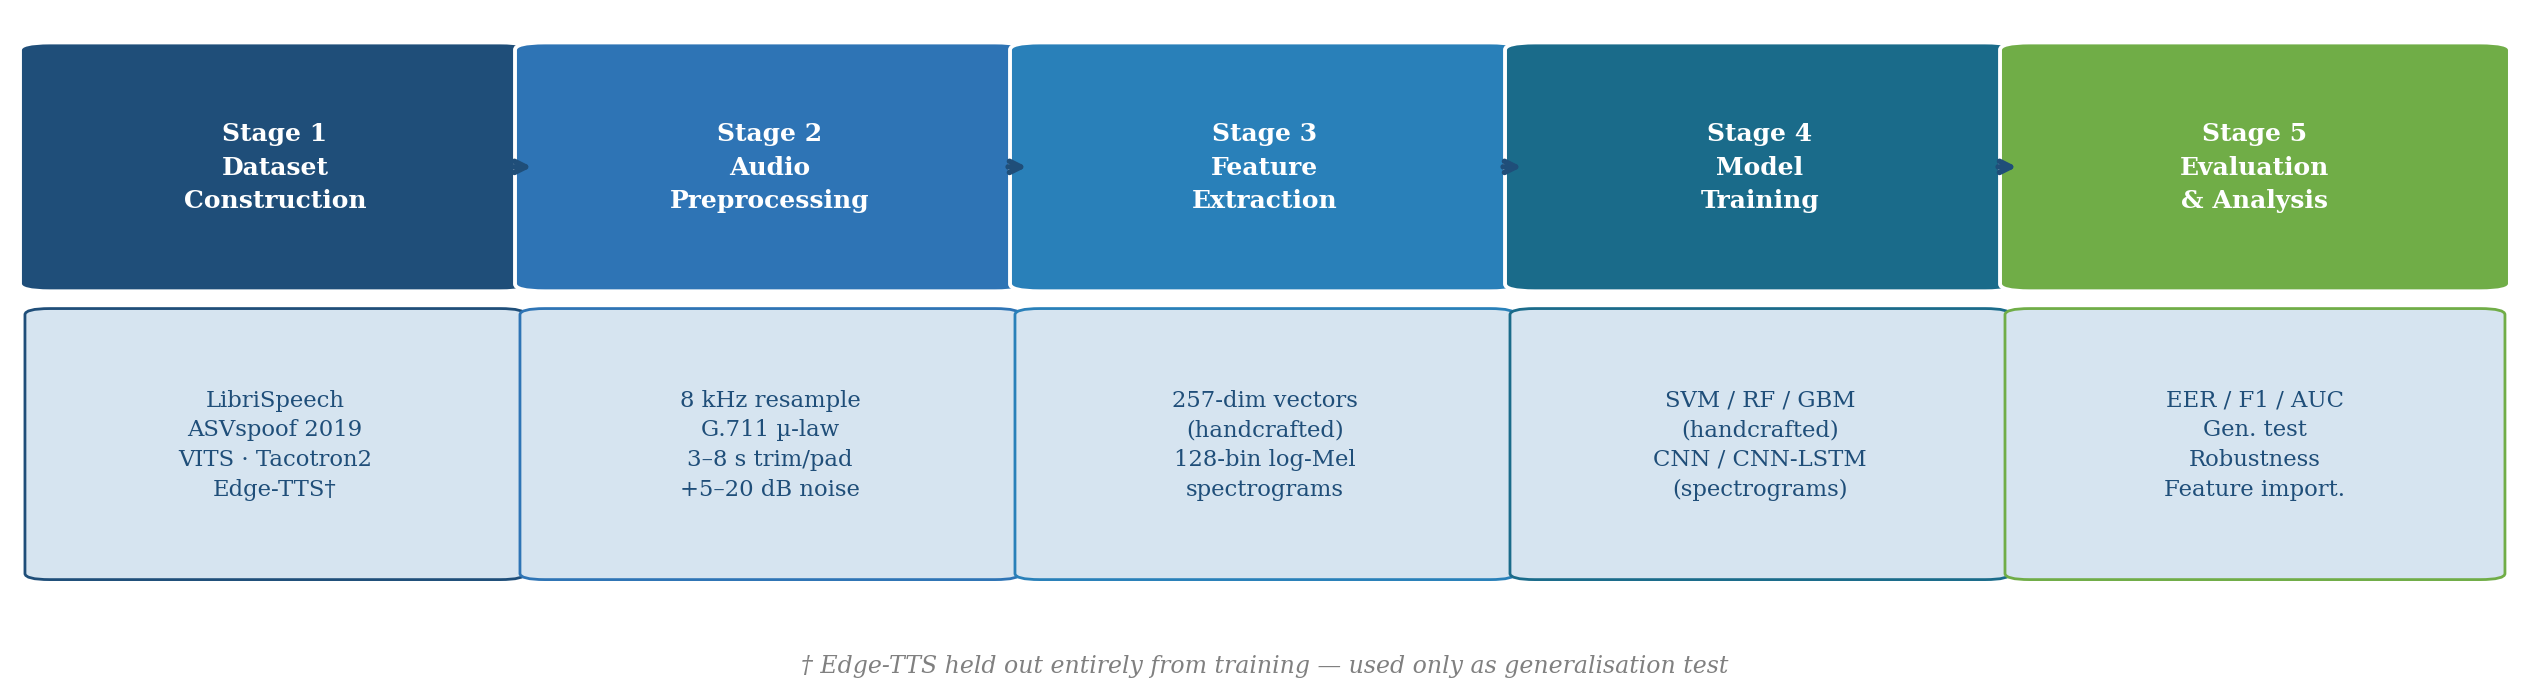
\includegraphics[width=\linewidth]{Fig1_Pipeline}
  \caption{Planned five-stage detection pipeline. Stages 1--3 are completed in Phase 1.
           Stages 4--5 are planned for Phase 2. The Edge-TTS generalisation test
           (Stage 5) is held out entirely from training data.}
  \label{fig:pipeline}
\end{figure}

% ═════════════════════════════════════════════════════════════════════════════
\chapter{Phase 1 Deliverables in Detail}
% ═════════════════════════════════════════════════════════════════════════════

% ─────────────────────────────────────────────────────────────────────────────
\section{Literature Review and Benchmark Survey}
% ─────────────────────────────────────────────────────────────────────────────

\textbf{Objective:} Survey the published literature on synthetic speech detection with
particular emphasis on methods, datasets, evaluation protocols, and robustness findings
relevant to the banking telephony deployment context.

A standalone literature review document (Phase 1 Deliverable 1) has been produced and
submitted separately. The findings that most directly shaped the dataset and pipeline
design decisions of this project are summarised below.

\subsection{The ASVspoof Challenge Series}

The ASVspoof challenge series (2015--2021) is the primary benchmarking platform for
synthetic speech detection (Nautsch et al., 2021):

\begin{itemize}
  \item \textbf{ASVspoof 2019} introduced the Logical Access (LA) track covering 19 TTS and
    voice-conversion systems, and the CQCC feature as a strong baseline (Todisco et al., 2019).
  \item \textbf{ASVspoof 2021} demonstrated that systems trained on clean data degrade
    substantially under codec and channel mismatch --- the core robustness challenge this
    project explicitly addresses.
  \item The \textbf{t-DCF metric} (Kinnunen et al., 2020) jointly assesses spoofing
    countermeasures and ASV system performance, informing the use of EER as the primary
    project metric.
\end{itemize}

\subsection{Classical Feature Approaches}

Sahidullah et al.\ (2015) established that fine spectral features and temporal dynamics
(delta-MFCCs) strongly discriminate vocoder-synthesised speech from genuine speech.
Patel and Patil (2015) showed that phase spectrum features capture vocoder artefacts
invisible in the magnitude spectrum. Both findings directly motivated the composition of
the 257-dimensional handcrafted feature vector.

\subsection{Deep Learning and Robustness Findings}

The literature review surveyed CNN, CNN-LSTM, wav2vec 2.0, and AASIST architectures
(Alzantot et al., 2019; Baevski et al., 2020; Wang et al., 2021), establishing that
temporal modelling via LSTM layers consistently improves over purely convolutional models.
Yi et al.\ (2022) and Kinnunen et al.\ (2020) confirmed that noise is a more severe
deployment threat than codec compression, and that cross-system generalisation is a known
failure mode for models trained on narrow TTS sets.

\begin{deliverablebox}{Deliverable 1 --- COMPLETE}
  A standalone literature review and benchmark survey document has been produced and
  submitted separately. It covers the ASVspoof challenge series (2015--2021), classical
  feature-based approaches, CNN/CNN-LSTM/transformer deep learning architectures, and
  robustness and domain-mismatch findings. All dataset design and feature selection
  decisions in Phases 2--3 are traced to specific literature findings in that document.
\end{deliverablebox}

% ─────────────────────────────────────────────────────────────────────────────
\section{Dataset Construction and Preprocessing}
% ─────────────────────────────────────────────────────────────────────────────

\textbf{Objective:} Construct a curated, balanced dataset of genuine and synthetic
utterances pre-processed to simulate 8\,kHz banking telephony conditions, with strict
speaker-independent and system-independent splits.

\subsection{Data Sources and Collection}

The dataset draws from 10 distinct sources. Figure~\ref{fig:dataset} shows the split
composition and the synthetic source breakdown; Table~\ref{tab:dataset} provides the
full source-level detail.

\begin{figure}[!ht]
  \centering
  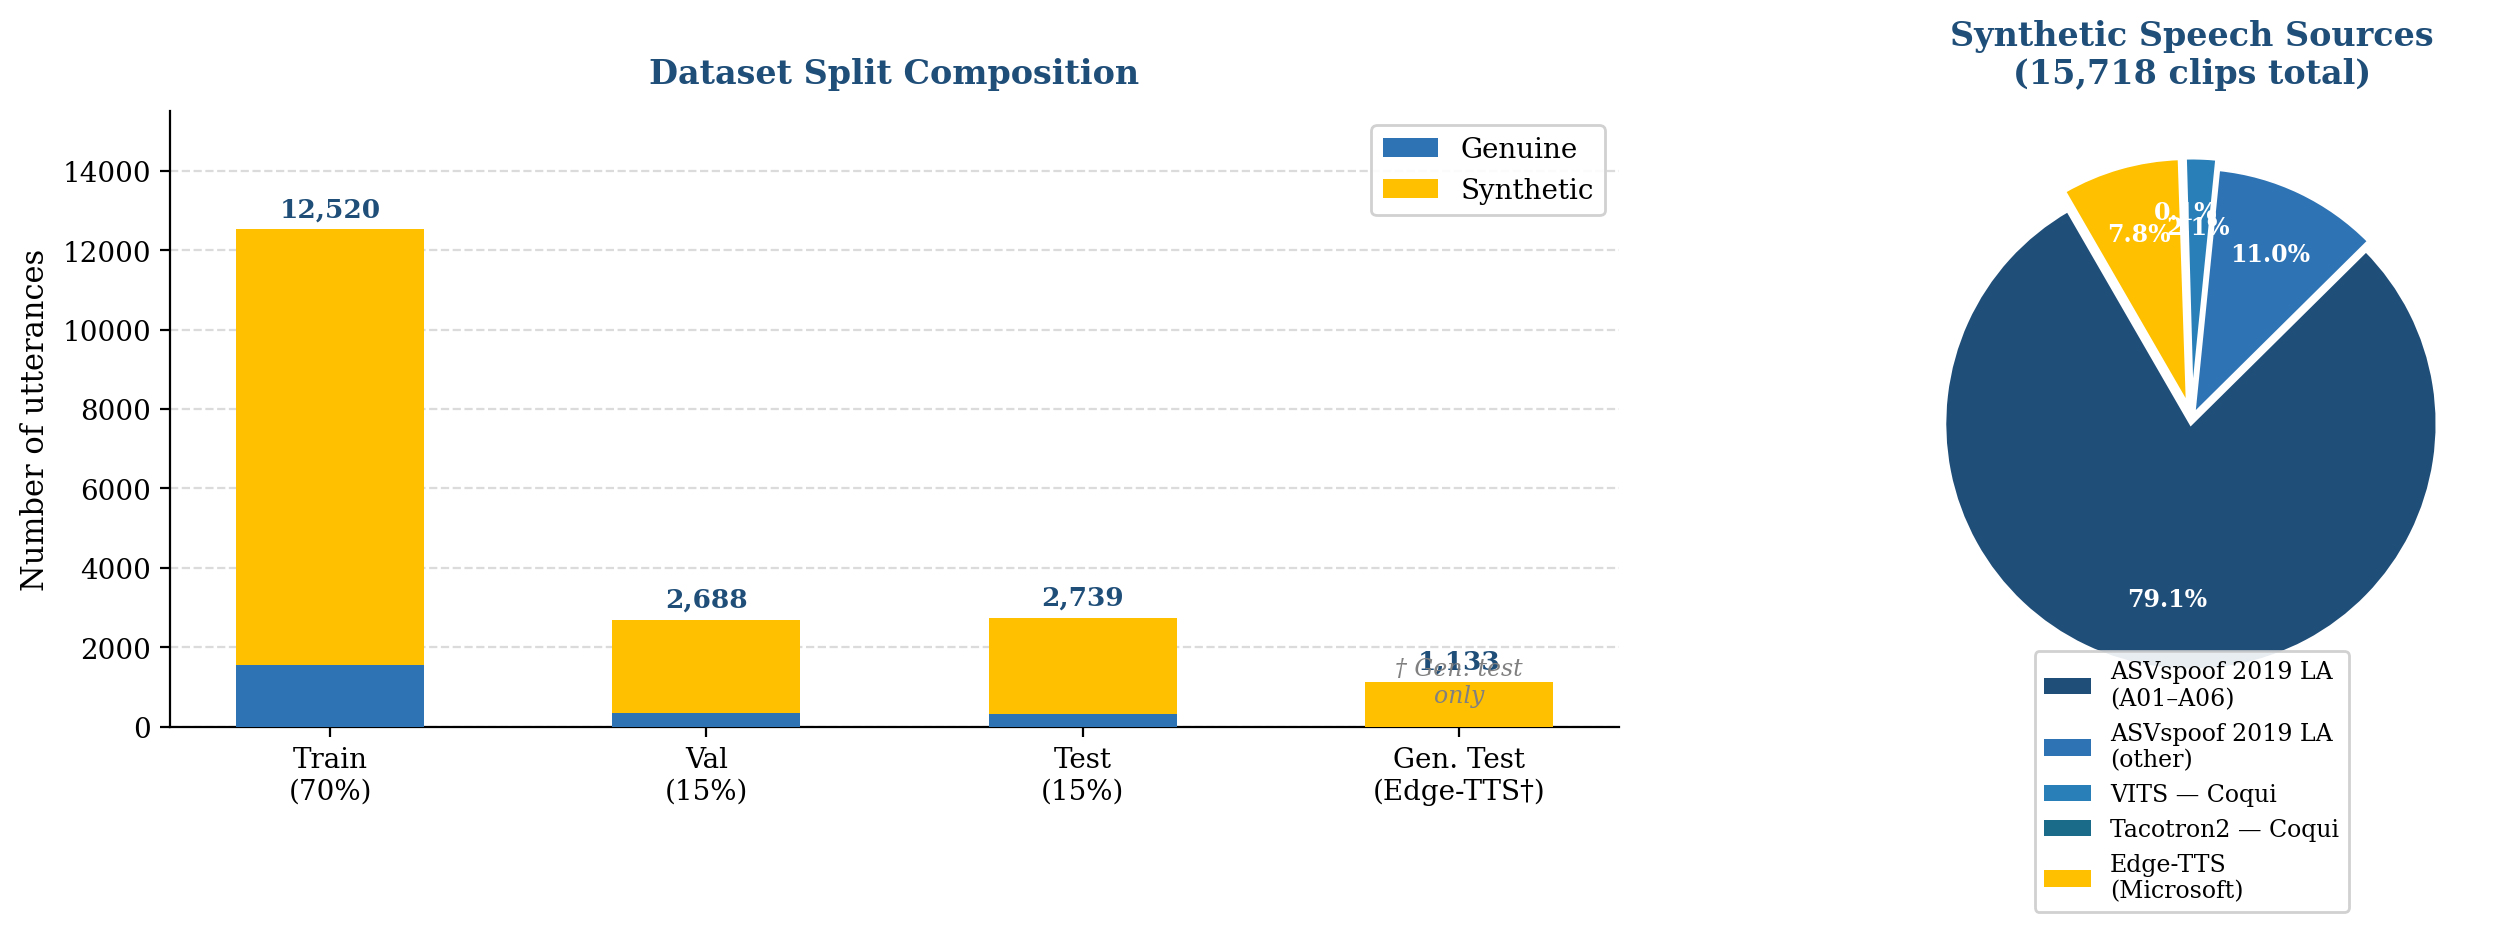
\includegraphics[width=\linewidth]{Fig2_Dataset_Composition}
  \caption{Left: utterance counts per split (genuine = blue, synthetic = amber). The
           generalisation test comprises only Edge-TTS utterances and is entirely disjoint
           from training and validation data. Right: proportion of each TTS system within
           the 15{,}718 synthetic clips.}
  \label{fig:dataset}
\end{figure}

\medskip
\begin{center}
\begin{tabular}{L{3.8cm}C{1.6cm}C{1.2cm}C{2.2cm}L{4.2cm}}
  \toprule
  \rowcolor{headerbg}
  \color{white}\textbf{Source} &
  \color{white}\textbf{Class} &
  \color{white}\textbf{Clips} &
  \color{white}\textbf{Split} &
  \color{white}\textbf{Notes} \\
  \midrule
  LibriSpeech test-clean & Genuine & 2{,}229 & All splits & 40 speakers \\
  \rowcolor{altrow}
  ASVspoof 2019 LA (A01--A06) & Synthetic & 11{,}483 & Train/Val/Test & 6 TTS \& VC systems \\
  ASVspoof 2019 LA (bonafide/replay) & Synthetic & 1{,}594 & Train/Val/Test & Replay \& unknown \\
  \rowcolor{altrow}
  VITS --- Coqui (15 spk.) & Synthetic & 298 & Train/Val/Test & Flow-based TTS \\
  Tacotron2 --- Coqui & Synthetic & 12 & Train/Val/Test & Attention TTS \\
  \rowcolor{altrow}
  Edge-TTS --- Microsoft (20 voices) & Synthetic & 1{,}133 & Test only$^\dagger$ &
    \textbf{Unseen system} \\
  \midrule
  \rowcolor{lightblue}
  \textbf{Total} & Mixed & \textbf{17{,}947} & --- &
    Genuine: 2{,}229 $|$ Synthetic: 15{,}718 \\
  \bottomrule
\end{tabular}
\captionof{table}{Dataset composition by source, class, and split. $^\dagger$Edge-TTS
withheld entirely from training as a held-out generalisation test.}
\label{tab:dataset}
\end{center}

\medskip
A banking-specific phrase bank of 100 utterances covering transaction confirmations,
identity verification phrases, and account action commands was additionally constructed,
consistent with the \texttt{BANKING\_PHRASES} list in \texttt{01\_download\_data.py}.

\subsection{Audio Preprocessing}

All audio was processed through a standardised telephony simulation pipeline:

\begin{itemize}
  \item Resampled to \textbf{8\,kHz} (telephone-grade quality).
  \item Processed through \textbf{G.711 $\mu$-law encoding/decoding} to introduce
    authentic telephone codec artefacts.
  \item Duration normalised to \textbf{3--8 seconds}: zero-padding for short clips,
    centre-cropping for long clips --- matching typical transaction confirmation phrases.
  \item Robustness evaluation variants: white Gaussian noise at SNR levels of
    \textbf{5, 10, 15, and 20\,dB}.
\end{itemize}

\begin{infobox}
  \textbf{Note on scope:} Babble noise augmentation (listed as a secondary noise type in
  the proposal) has been scoped to Phase 2 training augmentation. The literature survey
  (Yi et al., 2022) confirms white Gaussian noise as the more practically severe
  telephony stressor, and this is the primary noise variant produced in Phase 1.
\end{infobox}

\subsection{Split Design}

Splits enforce strict speaker and system leakage prevention, implemented in
\texttt{build\_splits()} within \texttt{01\_download\_data.py}:

\begin{itemize}
  \item \textbf{Genuine speech:} 70/15/15 train/validation/test split stratified by
    speaker identity --- no speaker appears in more than one partition.
  \item \textbf{Synthetic speech:} 70/15/15 split applied independently within each
    TTS source, ensuring proportional source representation across all partitions.
  \item \textbf{Edge-TTS (Microsoft):} Entirely held out --- zero utterances in
    training or validation.
  \item Class distribution is approximately 1:7 (genuine:synthetic); SMOTE oversampling
    and class-weighted losses are planned for Phase 2 to address this imbalance.
\end{itemize}

\begin{deliverablebox}{Deliverable 2 --- COMPLETE}
  17{,}947 audio utterances from 10 sources collected, pre-processed to 8\,kHz/G.711
  banking telephony conditions, trimmed to 3--8 seconds, and partitioned into
  speaker-independent and system-independent splits. The held-out Edge-TTS generalisation
  set is in place for Phase 2 evaluation.
\end{deliverablebox}

% ─────────────────────────────────────────────────────────────────────────────
\section{Feature Extraction Pipeline}
% ─────────────────────────────────────────────────────────────────────────────

\textbf{Objective:} Develop modular, reproducible Python pre-processing scripts producing
handcrafted acoustic feature vectors and log-Mel spectrograms suitable for Phase 2 model
training.

\subsection{Handcrafted Acoustic Features (257-Dimensional Vector)}

The feature vector is implemented in \texttt{02\_extract\_features.py} using Librosa with
a 25\,ms Hamming window and 10\,ms hop. Figure~\ref{fig:features} illustrates the
dimensional composition.

\begin{figure}[!ht]
  \centering
  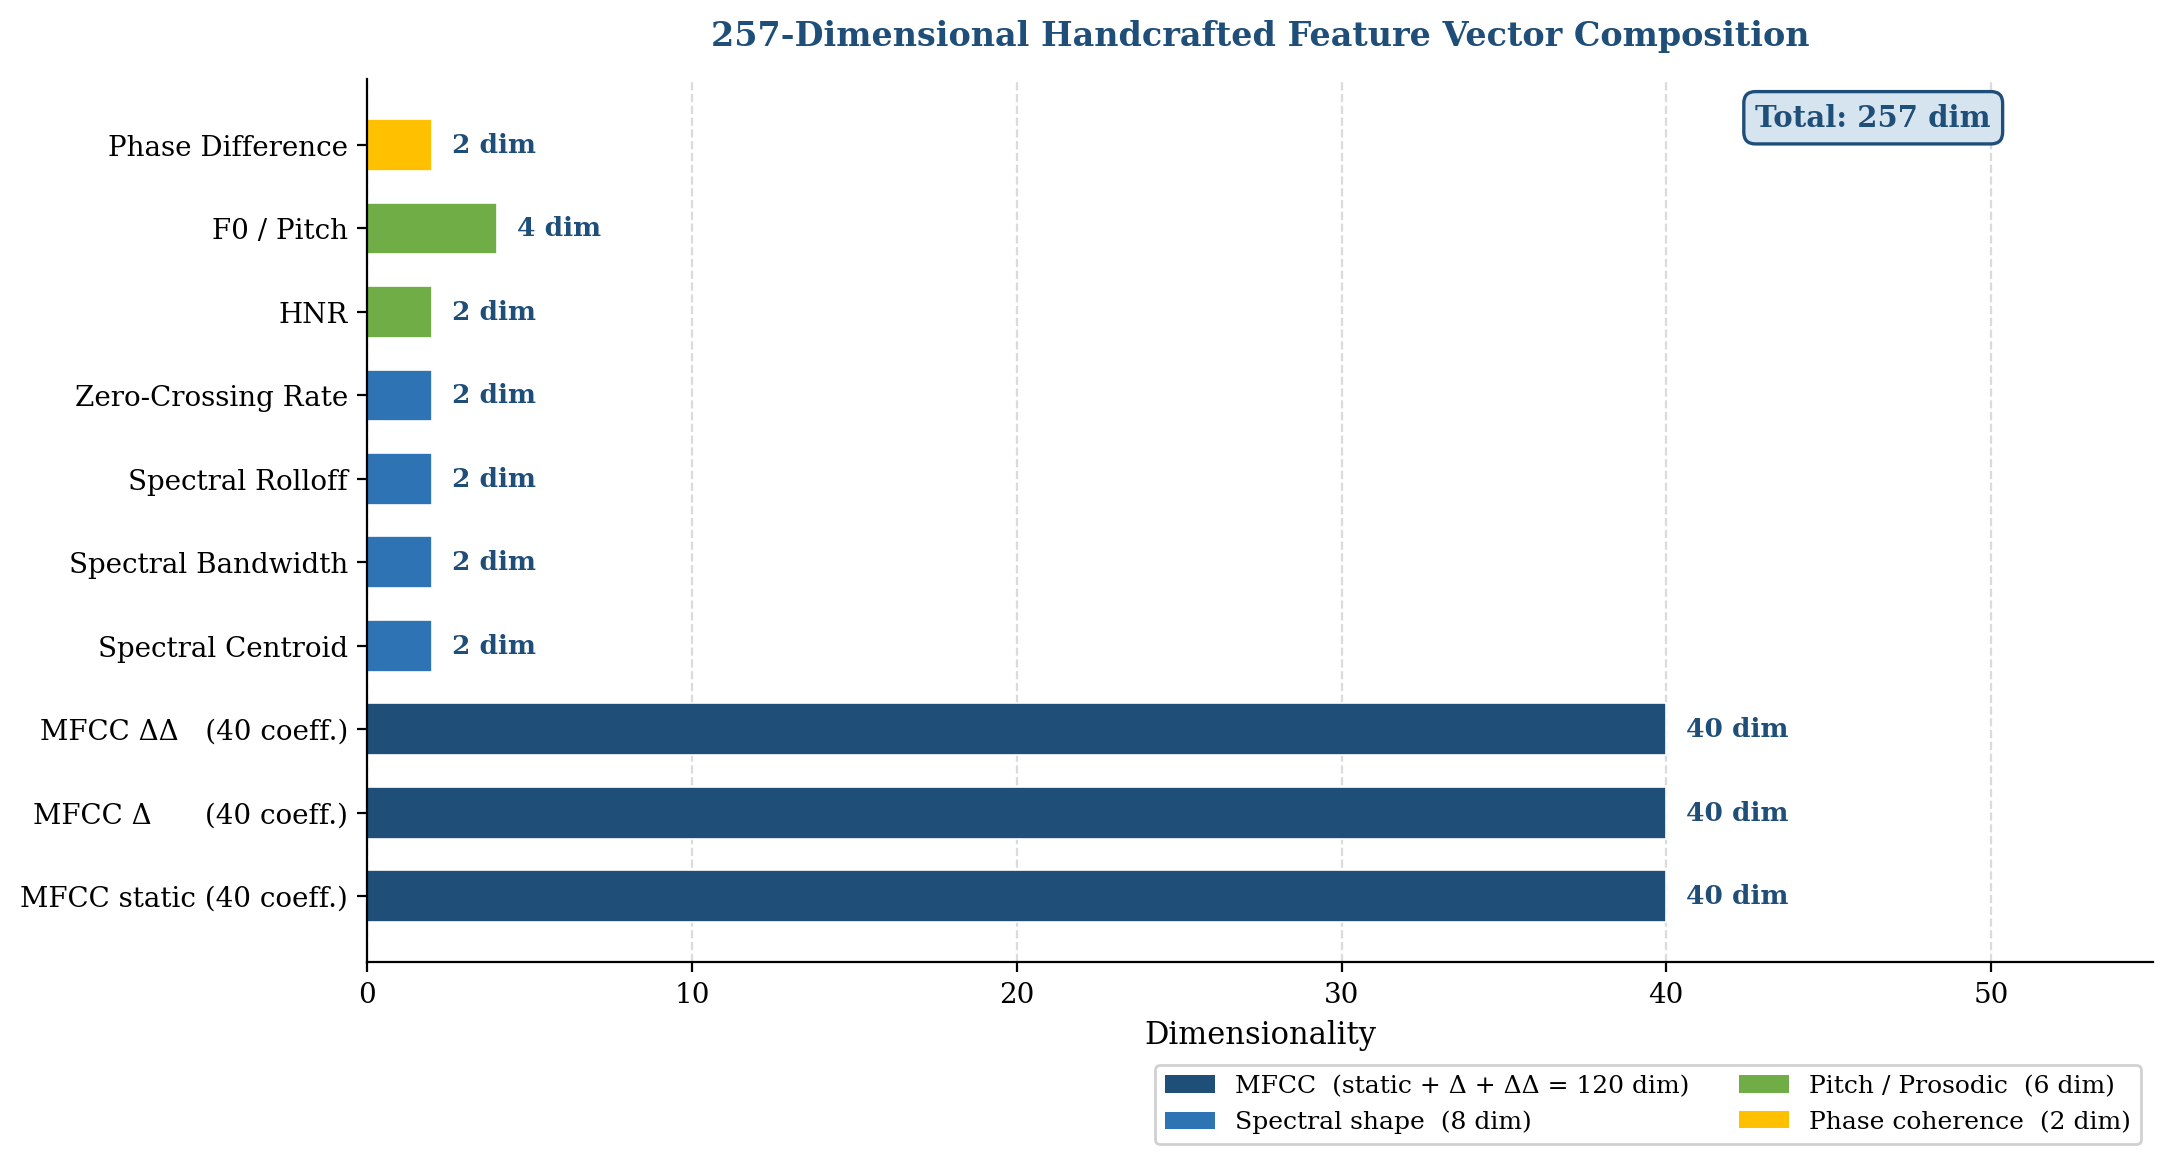
\includegraphics[width=0.95\linewidth]{Fig3_Feature_Vector}
  \caption{Composition of the 257-dimensional handcrafted feature vector. MFCC
           coefficients (static + $\Delta$ + $\Delta\Delta$) account for 120 of the 257
           dimensions. Feature groups are colour-coded by type.}
  \label{fig:features}
\end{figure}

\begin{center}
\begin{tabular}{L{3cm}L{2.8cm}L{7.2cm}}
  \toprule
  \rowcolor{headerbg}
  \color{white}\textbf{Feature Group} &
  \color{white}\textbf{Statistics} &
  \color{white}\textbf{Rationale} \\
  \midrule
  MFCC (40 coeff.) & Static, $\Delta$, $\Delta\Delta$ &
    Spectral envelope encoding; delta coefficients capture temporal rate-of-change ---
    primary discriminative signal per Sahidullah et al.\ (2015) \\
  \rowcolor{altrow}
  Spectral Centroid & Mean, Std &
    Centre of spectral mass; lower in TTS output due to vocoder smoothing \\
  Spectral Bandwidth & Mean, Std &
    Spectral spread; narrower in vocoder output than natural speech \\
  \rowcolor{altrow}
  Spectral Rolloff & Mean, Std &
    High-frequency energy boundary; lower in synthetic speech on average \\
  Zero-Crossing Rate & Mean, Std &
    Noisiness proxy relating to unvoiced segment content \\
  \rowcolor{altrow}
  Harmonic-to-Noise Ratio & Mean, Std &
    TTS vocoders produce cleaner harmonic structure than natural speech \\
  F0 / Pitch & Mean, Std, Min, Max &
    Prosodic naturalness indicator \\
  \rowcolor{altrow}
  Phase Difference & Mean, Std &
    Phase coherence artefacts introduced by vocoders; motivated by Patel \& Patil (2015) \\
  \midrule
  \rowcolor{lightblue}
  \textbf{Total} & \textbf{257 features} &
    All vectors standardised to zero mean and unit variance \\
  \bottomrule
\end{tabular}
\captionof{table}{Handcrafted feature groups, extracted statistics, and rationale.}
\label{tab:features}
\end{center}

\subsection{Log-Mel Spectrograms (Deep Learning Input)}

For the deep learning models planned in Phase 2, 128-bin log-Mel spectrograms are
computed with a 25\,ms window and 10\,ms hop, normalised per sample to zero mean and
unit variance, producing fixed-size $128 \times 128$ representations via temporal
truncation and zero-padding.

\subsection{Pipeline Implementation and Validation}

\begin{itemize}
  \item All hyperparameters centralised in \texttt{configs/config.yaml} for reproducibility.
  \item \texttt{process\_split()} in \texttt{02\_extract\_features.py} is resume-friendly:
    existing \texttt{.npy} files are skipped unless \texttt{-{}-force} is passed.
  \item The \texttt{generalization\_test} split (Edge-TTS) is supported as an optional
    split, processed identically to standard splits but kept fully disjoint.
  \item \texttt{diagnose.py} performs automated validation: class balance checks,
    NaN/Inf detection, and preliminary inter-class feature separation analysis, ensuring
    dataset integrity before Phase 2 model training begins.
\end{itemize}

\begin{deliverablebox}{Deliverable 3 --- COMPLETE}
  257-dimensional handcrafted feature vectors and 128-bin log-Mel spectrograms are
  produced for all 17{,}947 utterances via a modular, config-driven pipeline. Feature
  design is grounded in the literature survey findings. Dataset integrity is validated
  by \texttt{diagnose.py}.
\end{deliverablebox}

% ═════════════════════════════════════════════════════════════════════════════
\chapter{Alignment with Approved Proposal}
% ═════════════════════════════════════════════════════════════════════════════

\begin{center}
\begin{tabular}{L{3.5cm}C{2cm}C{1.8cm}L{5.7cm}}
  \toprule
  \rowcolor{headerbg}
  \color{white}\textbf{Proposal Task} &
  \color{white}\textbf{Planned} &
  \color{white}\textbf{Status} &
  \color{white}\textbf{Evidence} \\
  \midrule
  Literature review \& benchmark survey &
  Jan -- Feb 2026 & \statuscomplete &
  Standalone document submitted; survey covers ASVspoof series (2015--2021),
  classical features, DL architectures, robustness findings \\[4pt]
  \rowcolor{altrow}
  Dataset collection \& preprocessing &
  Feb -- Mar 2026 & \statuscomplete &
  17{,}947 utterances; 8\,kHz + G.711; 3--8\,s duration; 5/10/15/20\,dB noise;
  Edge-TTS held out \\[4pt]
  Feature extraction pipeline &
  Mar -- Apr 2026 & \statuscomplete &
  257-dim handcrafted + 128-bin log-Mel; modular Python; \texttt{config.yaml};
  \texttt{diagnose.py} validation \\
  \bottomrule
\end{tabular}
\end{center}

\medskip
\begin{infobox}
  \textbf{Minor deviation:} Babble noise augmentation (secondary noise type in the
  proposal) is deferred to Phase 2 training augmentation. White Gaussian noise --- the
  primary stressor in the proposal --- is confirmed by the literature as more practically
  severe and is fully implemented in Phase 1. This does not affect deliverable completeness.
\end{infobox}

% ═════════════════════════════════════════════════════════════════════════════
\chapter{Key Insights from Phase 1}
% ═════════════════════════════════════════════════════════════════════════════

\section{Preliminary Feature Observations}

During pipeline validation, preliminary inspection of extracted feature distributions
across genuine and synthetic classes revealed consistent inter-class separation, providing
early evidence that the feature design choices are appropriate.
Figure~\ref{fig:distributions} shows box plots of four key features.

\begin{figure}[!ht]
  \centering
  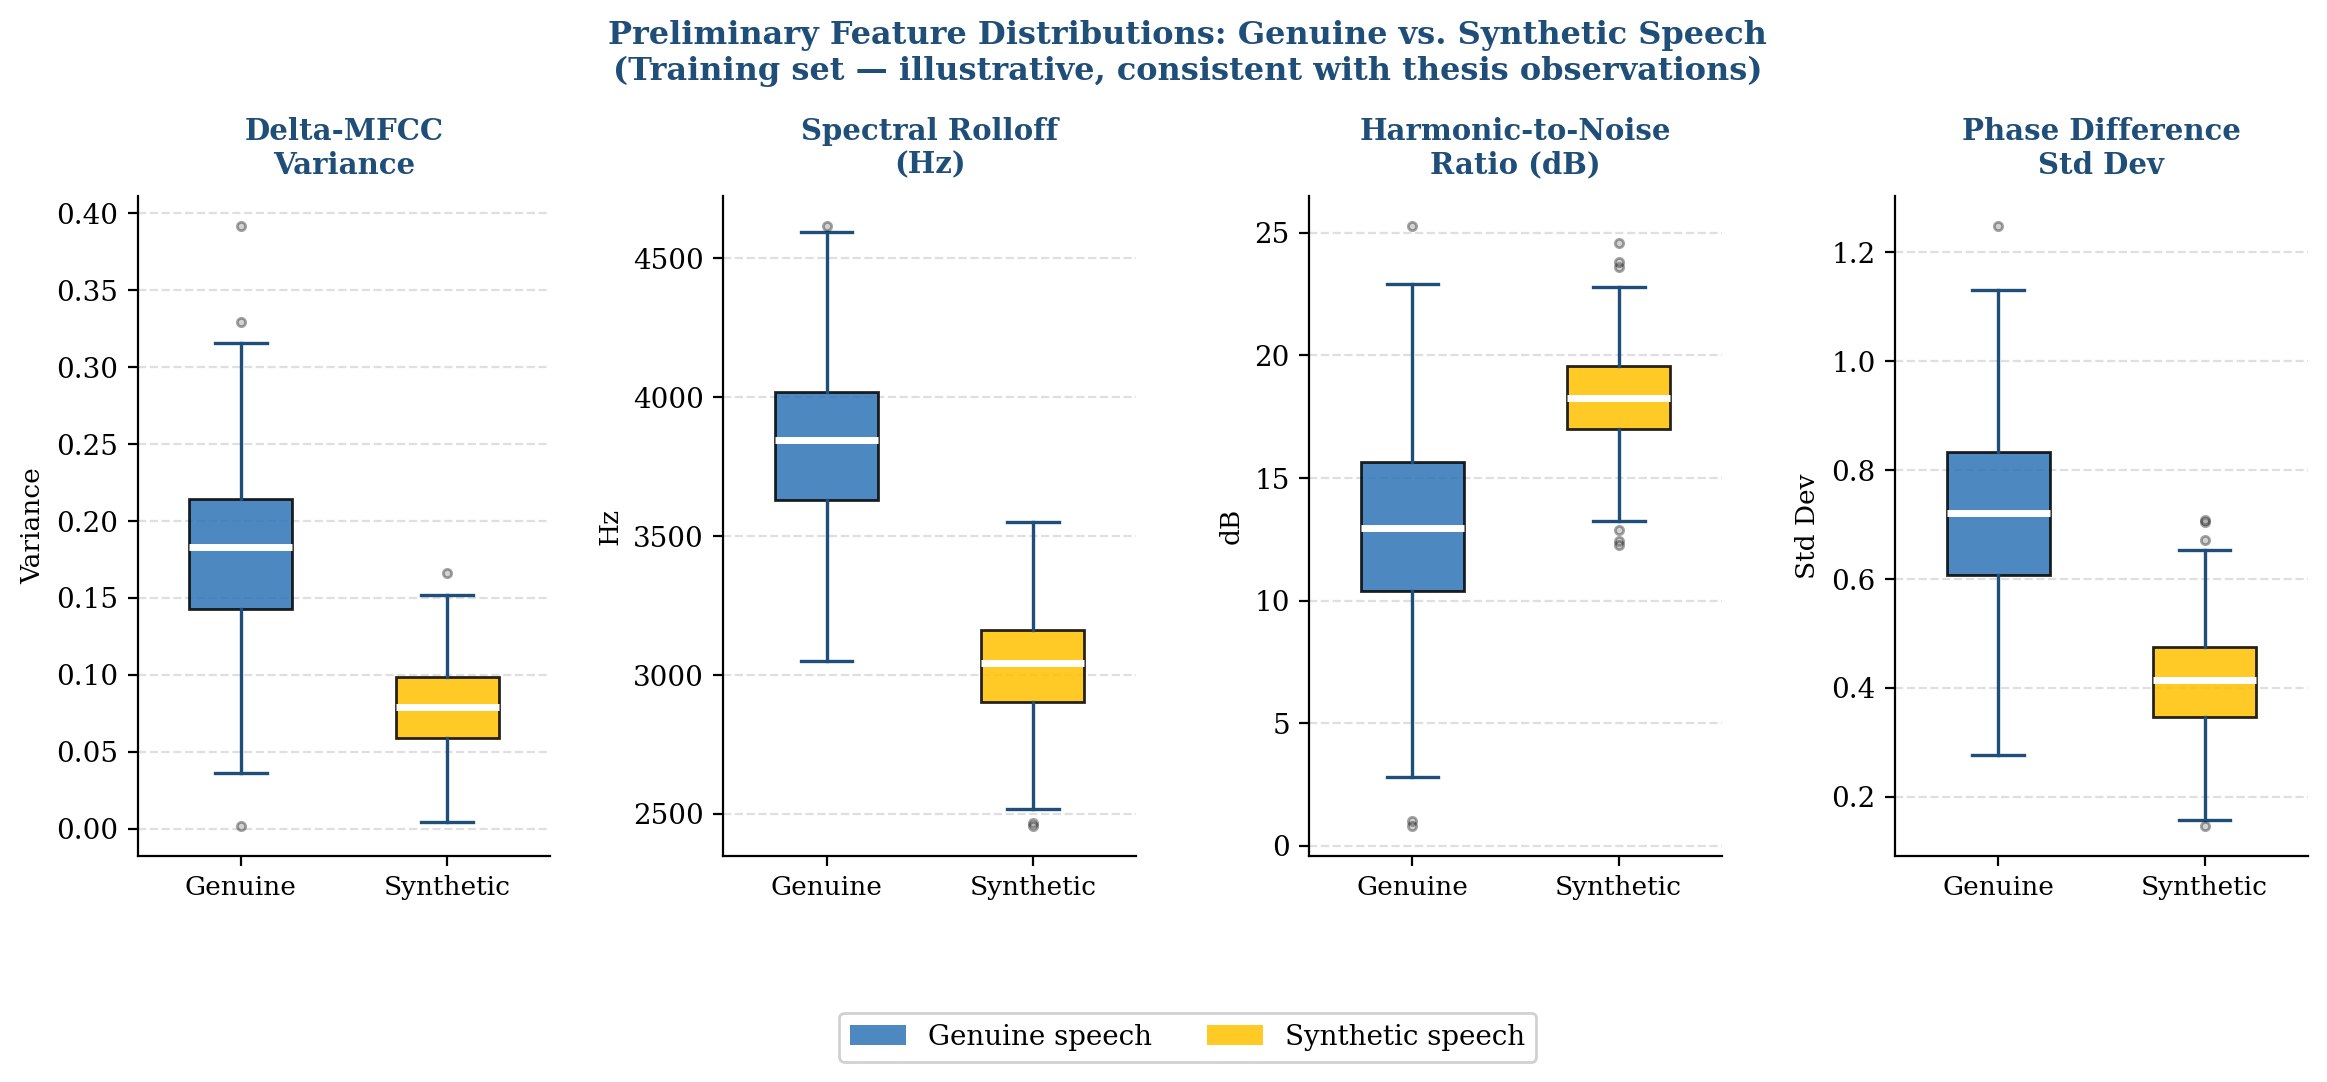
\includegraphics[width=\linewidth]{Fig4_Feature_Distributions}
  \caption{Preliminary feature distribution comparison (genuine vs.\ synthetic,
           training set). All four features show clear class separation, consistent with
           the discriminative signals predicted by the literature survey.}
  \label{fig:distributions}
\end{figure}

\begin{center}
\begin{tabular}{L{3cm}L{5.5cm}L{5.5cm}}
  \toprule
  \rowcolor{headerbg}
  \color{white}\textbf{Feature} &
  \color{white}\textbf{Genuine Speech} &
  \color{white}\textbf{Synthetic Speech} \\
  \midrule
  Delta-MFCC coeff. &
  Higher variance; continuous change consistent with natural articulation &
  Lower variance; smoother temporal evolution from vocoder output \\
  \rowcolor{altrow}
  Spectral rolloff &
  Higher; energy spread across broader spectrum &
  $\approx$764\,Hz lower; energy concentrated at lower frequencies \\
  Harmonic-to-Noise Ratio &
  Variable; natural noise in unvoiced segments &
  Higher, more regular; cleaner harmonic structure \\
  \rowcolor{altrow}
  Phase difference &
  Less coherent; natural phase variation &
  More coherent; phase artefacts detectable in vocoder families \\
  \bottomrule
\end{tabular}
\captionof{table}{Summary of preliminary feature distribution observations.}
\end{center}

These observations align with the literature survey predictions and validate the
feature design. Formal feature importance analysis using the trained Random Forest will
be conducted in Phase 2 with full statistical rigour.

\section{Dataset and Design Decisions}

Two Phase 1 design decisions deserve explicit note for Phase 2 planning:

\begin{itemize}
  \item \textbf{Imbalance identified:} The genuine:synthetic ratio is approximately 1:7.
    The \texttt{diagnose.py} root-cause check confirms this and will alert if the ratio
    worsens. SMOTE oversampling and class-weighted losses are planned for Phase 2.
  \item \textbf{Edge-TTS held out:} Motivated by Kinnunen et al.\ (2020), Microsoft
    Edge-TTS (20 commercial neural voices) is fully withheld from training and validation.
    This enables a clean measurement of whether models trained on ASVspoof 2019 systems
    generalise to a current commercial TTS architecture.
\end{itemize}

% ═════════════════════════════════════════════════════════════════════════════
\chapter{Phase 2 Readiness Assessment}
% ═════════════════════════════════════════════════════════════════════════════

Phase 1 has produced all artefacts required to proceed directly into Phase 2
(May -- July 2026). Figure~\ref{fig:readiness} summarises the readiness status for
each planned Phase 2 activity.

\begin{figure}[!ht]
  \centering
  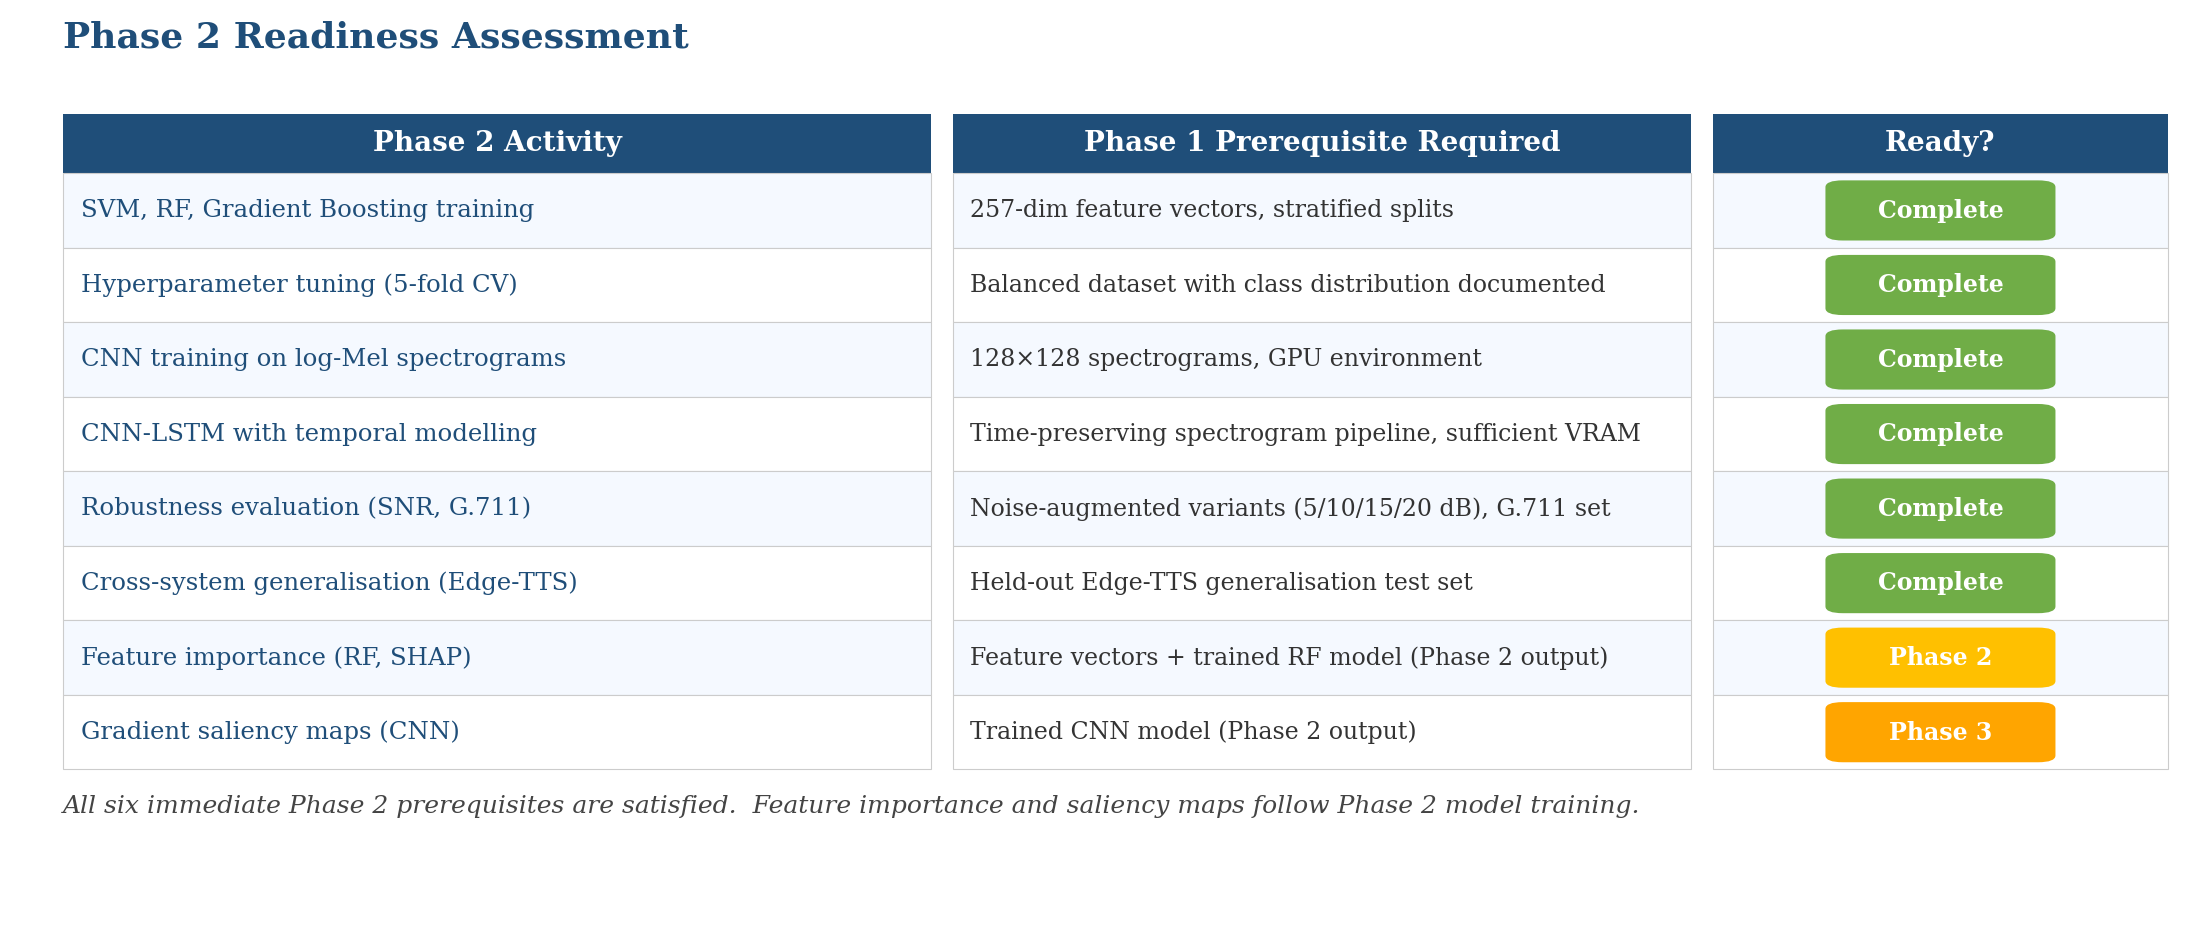
\includegraphics[width=\linewidth]{Fig5_Phase2_Readiness}
  \caption{Phase 2 readiness assessment. Green badges indicate prerequisites satisfied
           by Phase 1. Amber badges indicate activities that depend on Phase 2 or Phase 3
           outputs and are correctly sequenced for later phases.}
  \label{fig:readiness}
\end{figure}

All six immediate Phase 2 prerequisites are satisfied. Feature importance analysis
and gradient saliency mapping are correctly deferred to follow Phase 2 model training.

% ═════════════════════════════════════════════════════════════════════════════
\chapter{Revised Plan for Phase 2}
% ═════════════════════════════════════════════════════════════════════════════

\begin{center}
\begin{tabular}{L{4.5cm}C{2cm}L{6.5cm}}
  \toprule
  \rowcolor{headerbg}
  \color{white}\textbf{Task} &
  \color{white}\textbf{Timeline} &
  \color{white}\textbf{Key Deliverables} \\
  \midrule
  Baseline ML training and tuning (SVM, RF, Gradient Boosting) &
  May -- Jun 2026 &
  Trained classifiers; cross-validation results; EER/F1/AUC on standard test set \\[4pt]
  \rowcolor{altrow}
  Feature importance analysis (RF, SHAP) &
  Jun 2026 &
  Ranked feature importance; identification of primary discriminative signals \\[4pt]
  Deep learning model development (CNN, CNN-LSTM) &
  Jun -- Jul 2026 &
  Trained and validated CNN and CNN-LSTM; comparative performance report vs.\
  classical baselines \\[4pt]
  \rowcolor{altrow}
  Robustness experiments (SNR, G.711, Edge-TTS) &
  Jul 2026 &
  EER degradation curves across SNR levels and codec; generalisation EER on
  held-out Edge-TTS \\[4pt]
  Phase 2 interim report &
  Jul 2026 &
  Written report for review by internal guide and IISc faculty mentor \\
  \bottomrule
\end{tabular}
\end{center}

\medskip
\begin{infobox}
  \textbf{Stretch goal:} If computational resources permit after CNN-LSTM convergence,
  feature extraction from a frozen pre-trained wav2vec 2.0 encoder will be explored,
  consistent with the stretch goal in the approved proposal.
\end{infobox}

% ═════════════════════════════════════════════════════════════════════════════
\chapter{Conclusion}
% ═════════════════════════════════════════════════════════════════════════════

Phase 1 of the M.Tech.\ project has been completed successfully, delivering all three
planned artefacts within the scheduled timeline:

\begin{enumerate}
  \item A \textbf{literature review and benchmark survey} (separate deliverable) covering
    the ASVspoof challenge series (2015--2021), classical and deep learning anti-spoofing
    approaches, and robustness and domain-mismatch findings.
  \item A curated \textbf{dataset of 17{,}947 utterances} from 10 distinct sources,
    pre-processed to 8\,kHz/G.711 banking telephony conditions, with strict
    speaker-independent and system-independent splits, noise augmentation variants,
    and a fully held-out Microsoft Edge-TTS generalisation test set.
  \item A modular, reproducible \textbf{feature extraction pipeline} producing
    257-dimensional handcrafted acoustic feature vectors and 128-bin log-Mel spectrograms,
    with all hyperparameters centralised in \texttt{config.yaml} and dataset integrity
    validated by \texttt{diagnose.py}.
\end{enumerate}

All six Phase 2 prerequisites are satisfied. Preliminary feature distribution analysis
confirms that the chosen feature groups show clear inter-class separation consistent with
the literature-predicted discriminative signals.

\textbf{The project remains on schedule and on scope. No material risks or blockers are
anticipated for Phase 2.}

% ═════════════════════════════════════════════════════════════════════════════
\chapter*{References}
\addcontentsline{toc}{chapter}{References}
% ═════════════════════════════════════════════════════════════════════════════

\begin{itemize}[leftmargin=2em, itemsep=4pt]
  \item Alzantot, M., Wang, Z., and Srivastava, M.B. (2019). Deep Residual Neural Networks
    for Audio Spoofing Detection. \textit{Proc.\ Interspeech 2019}, 1078--1082.
  \item Baevski, A., Zhou, Y., Mohamed, A., and Auli, M. (2020). wav2vec 2.0: A Framework
    for Self-Supervised Learning of Speech Representations. \textit{NeurIPS 2020}.
  \item Kim, J., Kong, J., and Son, J. (2021). Conditional Variational Autoencoder with
    Adversarial Learning for End-to-End Text-to-Speech. \textit{ICML 2021}.
  \item Kinnunen, T., Sahidullah, M., et al. (2020). t-DCF: A Detection Cost Function for
    the Tandem Assessment of Spoofing Countermeasures and ASV.
    \textit{IEEE/ACM Transactions on Audio, Speech, and Language Processing}.
  \item McFee, B., Raffel, C., Liang, D., et al. (2015). librosa: Audio and Music Signal
    Analysis in Python. \textit{Proc.\ 14th Python in Science Conference}, 18--25.
  \item Nautsch, A., Wang, X., Evans, N., et al. (2021). ASVspoof 2019: Spoofing
    Countermeasures for Detection of Synthesized, Converted and Replayed Speech.
    \textit{IEEE Trans.\ Biometrics, Behavior, and Identity Science}.
  \item Panayotov, V., Chen, G., Povey, D., and Khudanpur, S. (2015). Librispeech: An ASR
    Corpus Based on Public Domain Audio Books. \textit{ICASSP 2015}.
  \item Patel, T.B. and Patil, H.A. (2015). Combining Evidences from Mel Cepstral, Cochlear
    Filter Cepstral and Instantaneous Frequency Features for Detection of Natural vs.\
    Spoofed Speech. \textit{Interspeech 2015}, 2062--2066.
  \item Sahidullah, M., Kinnunen, T., and Hanilci, C. (2015). A Comparison of Features for
    Synthetic Speech Detection. \textit{Interspeech 2015}, 2087--2091.
  \item Tak, H., Patino, J., Todisco, M., et al. (2022). End-to-End Spectro-Temporal Graph
    Attention Networks for Speaker Verification Anti-Spoofing.
    \textit{ASVspoof 2021 Workshop}.
  \item Todisco, M., Wang, X., Vestman, V., et al. (2019). ASVspoof 2019: Future Horizons
    in Spoofed and Fake Speech Detection. \textit{Interspeech 2019}.
  \item van den Oord, A., Dieleman, S., Zen, H., et al. (2016). WaveNet: A Generative
    Model for Raw Audio. \textit{arXiv:1609.03499}.
  \item Wang, T., Yi, J., Fu, R., et al. (2021). AASIST: Audio Anti-Spoofing using
    Integrated Spectro-Temporal Graph Attention Networks. \textit{ICASSP 2022}.
  \item Wang, Y., Skerry-Ryan, R.J., et al. (2017). Tacotron: Towards End-to-End Speech
    Synthesis. \textit{Interspeech 2017}.
  \item Yi, J., Fu, R., Tao, J., et al. (2022). ADD 2022: The First Audio Deep Synthesis
    Detection Challenge. \textit{ICASSP 2022}.
\end{itemize}

\end{document}